\setchapterpreamble[u]{\margintoc}
\chapter{Proof-by-Action in Practice}
\labch{advanced}

In the previous chapters, we explained the core principles of our so-called
Proof-by-Action paradigm and especially its drag-and-drop actions, first through
basic and abstract examples in \refch{pba}, and then from a proof-theoretical
perspective in \refch{sfl}. The goal of this chapter is to provide a better
sense of what proofs by action/DnD look like in practice, and how they compare
to more traditional approaches to interactive theorem proving. To that effect,
we perform a case study of a few select examples, unrolling and commenting in
details one or many of their proofs. Although still basic, they are fully
fledged, concrete logical riddles or mathematical problems that one might give
as exercise to an undergraduate student learning formal proofs. Note that our
analysis will stay quite informal and opinionated: a more systematic approach
such as a user study would allow for a better evaluation of our paradigm, but at
the time of writing of this thesis the Actema prototype is not mature enough to
conduct a project of this scale.

The chapter is organized as follows: \refsec{edukera} studies a proof of a small
logical riddle in Actema, highlighting some benefits of our approach compared to
textual systems. \refsec{funcs} explores how basic properties about functions
between sets can be proved graphically, introducing the use of definitions in
addition to logical reasoning steps. In \refsec{arith} we prove equations in
Peano arithmetic, showing how one can incorporate additional actions into the
paradigm to deal with more specialized forms of reasoning: \emph{induction} and
\emph{automatic computation}.

\todo{ Explain that for all examples, we provide a Coq proof script that tries
  to follow the structure of the graphical proof, for the sake of comparison
  with a more standard text-based interface. But this would obviously compare
  differently with other textual approaches, e.g. Isar which is more
  declarative, and thus farther from the Proof-by-Action paradigm. }

\todo{ Maybe advise the reader to reproduce the examples herself? Supposes an
  easy way to setup and use coq-actema: nix seems like a good option, but maybe
  JsCoq could be doable with some efforts, and would provide an even more
  out-of-the-box experience.}
  
\todo{ Real numbered equations for intermediate proof states. }

\section{Forward reasoning}\labsec{edukera}

% It is too early to perform a detailed case study comparing our approach
% to interactive theorem proving with others --- tactic-based,
% declarative, {\em etc}\dots~This is due primarily to the fact that
% our prototype is not mature enough; it cannot handle lemmas and
% implements a limited formalism. However some examples allow to get a
% glimpse of specificities and possible advantages of proofs by actions.

Our first example is a small logical riddle, which we borrow from a textual
educational system, Edukera~\sidecite{edukera}. One considers a population of
people, with at least one individual $h$, together with a single function
$\mother$ and one predicate $\rich$. The aim is to show that the two following
assumptions are incompatible:
\begin{itemize}
\item[(1)] $\forall x. \neg\rich(x)\lor \neg\rich(\mother(\mother(x)))$,
\item[(2)] $\forall x. \neg\rich(x) \limp \rich(\mother(x)).$
\end{itemize}
The original goal thus corresponds to the illustration of \reffig{edukera}.

\begin{figure*}
  \fbox{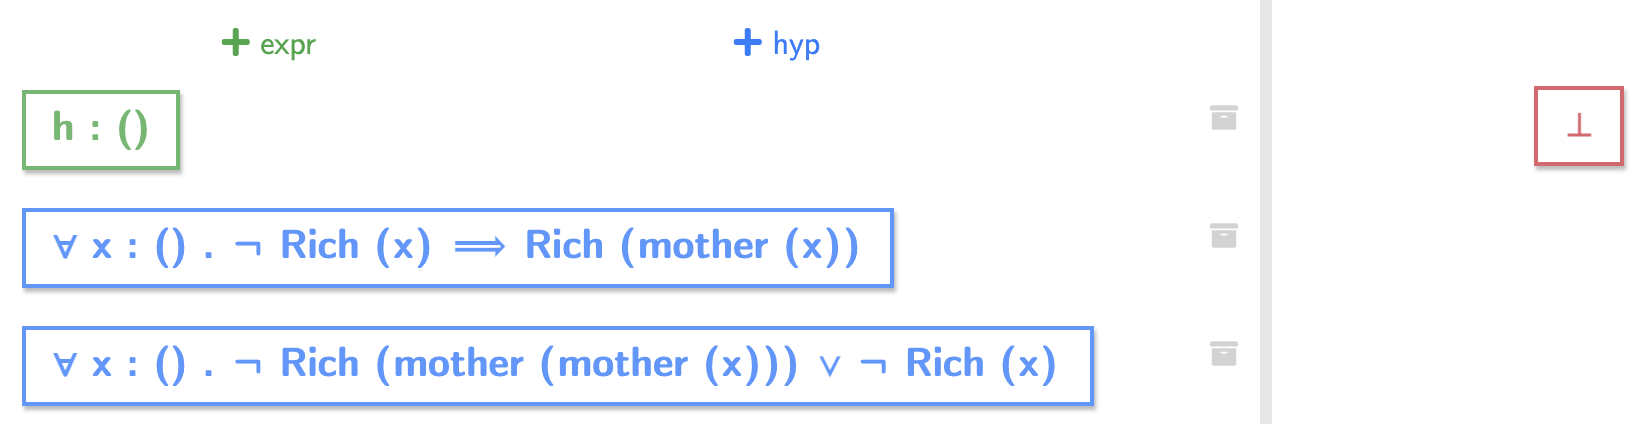
\includegraphics[width=1.3\textwidth]{edukera.png}}
  \caption{The beginning of an example due to Edukera}
  \labfig{edukera}
\end{figure*}

It is quite natural to approach this problem in a forward manner, by starting
from the hypotheses to establish new facts. And a first point illustrated by
this example is that DnD actions allow to do this in a smooth and precise
manner. A possible first step is to bring $h$ to the first hypothesis, to obtain
a new fact:

\medskip
$(3) ~\neg\rich(h)\lor \neg\rich(\mother(\mother(h))).$
\medskip

\noindent Double clicking on this new fact yields two cases:
\begin{itemize}
 \item[(4)~] $ \neg\rich(h)$,
 \item[(4')] $ \neg\rich(\mother(\mother(h)))$.
 \end{itemize}
Let us detail how one solves the
second one.

By bringing 
$\neg\rich(\mother(\mother(h)))$ on the premise of $\forall
x. \select{\neg\rich(x)} \limp \rich(\mother(x))$
one obtains

\medskip
$(6) ~\rich(\mother(\mother(\mother(h)))).$
\medskip

The next step is a good example where DnD actions are useful. By bringing this
new fact to the right-hand part of

\medskip
$(1)~\forall x. \neg\rich(x)\lor \neg\select{\rich(\mother(\mother(x)))}$
\medskip

\noindent
one immediately obtains a new fact

\medskip
$(7) ~\neg{\rich(\mother(h))}$.
\medskip

\noindent In other proof systems, this last step requires a somewhat intricate
tactic line and/or writing down at least the statement of the new fact.

One can then finish the case by combining $(7)$ and $(2)$ which yields
$$\rich(\mother(\mother(h)))$$ contradicting $(4')$. These two last steps each
correspond to a simple DnD. The other case, $\neg\rich(h)$, is quite similar.

% Such a simple example is not sufficient to provide significant metrics.
Note that once a user has understood the proof, the riddle is routinely solved
in less than a minute in Actema, which seems out of reach for about any user in
a tactic based prover. At least as important is the fact that the proof can be
performed without typing any text, especially no intermediate statement. 

To conclude this example, we propose in \reffig{edukera-coq} a complete proof of
the riddle formalized in the Coq proof assistant, which follows very closely the
structure of the graphical proof just outlined. To make the correspondence more
visible and ease the comparison, we interspersed the proof script with comments
of the form \texttt{(** [actions] *)}, where \texttt{[actions]} is a
sentence describing a sequence of actions in Actema that produces the same goal
transformation as the tactics preceding the comment. There are a few interesting
things to note:
\begin{itemize}
  \item We chose to name manually all the hypotheses introduced in the course of
  the proof. This is generally considered good practice in the Coq community,
  because it makes proof scripts easier to maintain. In our case it also has the
  advantage of expliciting which hypotheses are used exactly in the reasoning,
  something that an Actema user does with her pointing device when designating
  the blue items involved in an action. It appears clearly in
  \reffig{edukera-coq} that in a moderately long proof like this based mostly on
  forward reasoning, one needs to keep track of \emph{a lot} of names, which can
  be overwhelming for many users. This is especially true for beginners
  discovering Coq, because the syntax for assigning names, based on patterns
  like \texttt{[H | H]} that reproduce the subgoal structure, can induce a steep
  learning curve. Of course this problem is mitigated trivially in Actema, since
  names are not needed.

  \item There is no exact correspondence between the tactics of Coq and the
  actions of Actema: some tactics are simulated by multiple actions, and often a
  complex sequence of tactics can be simulated by a single action\sidenote{This
  was already noticed in \cite{PbP}, where clicking on a subformula can simulate
  a sequence of introduction rules of arbitrary length.}.
  
  For instance, line 23 does at the same time a specialization of the hypothesis
  $H_2 : \forall x. \neg \rich(\mother(\mother(x))) \lor \neg \rich(x)$ to the
  individual $h$ with the application \texttt{(H2 h)}, and a case analysis with
  the \texttt{destruct} tactic. In Actema this is performed in two steps, first
  by drag-and-dropping $h$ on $H_2$, and then by clicking on the resulting
  hypothesis\sidenote{This could also be achieved in two steps in Coq, by using
  the \texttt{specialize} tactic instead of the inlined application.}.

  In the other direction, a pattern of reasoning that occurs multiple times in
  the proof is the combination of $H_2$ with another hypothesis which
  contradicts one of the two cases, in order to deduce the truth of the other
  case. While it is captured straightforwardly in Actema with a single DnD
  between the contradictory statements, it requires in Coq a decomposition into
  many administrative steps:
  \begin{enumerate}
    \item first a case analysis with \texttt{destruct}, where the expression
    instantiating $H_2$ (e.g. $\mother(mother(h))$) needs to be written down
    explicitly, instead of being inferred automatically from unification;
    \item optionally focusing on the subgoal corresponding to the contradictory
    case if it is the right disjunct (line 56), which requires to know a
    somewhat idiosyncratic and infrequently used syntax of the tactic language;
    \item and finally expliciting the contradiction with \texttt{apply} and
    \texttt{exact}.
  \end{enumerate}

  \item More generally, the actions of Actema are more \emph{versatile} and
  \emph{context-dependent} than the tactics of Coq. For instance, click actions
  have a different effect depending on the main connective of the formula being
  clicked, but provide a unique interface for applying rules of natural
  deduction/sequent calculus. On the contrary, there is almost one tactic for
  dealing with each logical connective in Coq, e.g. \texttt{intros} for $\limp$
  and $\forall$, \texttt{split} for $\land$, \texttt{left} and \texttt{right}
  for $\lor$, \texttt{exists} for $\exists$, etc. The same remark applies to DnD
  actions, whose functionalities are provided in Coq by many different tactics:
  \texttt{apply \_}, \texttt{apply \_ in \_}, \texttt{pose proof},
  \texttt{specialize}, etc.
\end{itemize}

\begin{figure}
  % \fontsize{8}{8.5}\selectfont
  % \begin{alectryon}
  % Generator: Alectryon
  \sep
  \begin{txt}
    \PY{c}{(*~Declaration~of~constants~used~in~the~statement~of~the~riddle~*)}\nl
    \nl
  \end{txt}
  \sep
  \begin{sentence}
    \begin{input}
      \PY{k+kn}{Context}~\PY{o}{(}\PY{n+nv}{i}~\PY{o}{:}~\PY{k+kt}{Type}\PY{o}{).}\nl
    \end{input}
  \end{sentence}
  \sep
  \begin{txt}
    \nl
  \end{txt}
  \sep
  \begin{sentence}
    \begin{input}
      \PY{k+kn}{Context}~\PY{o}{(}\PY{n+nv}{Rich}~\PY{o}{:}~\PY{n}{i}~\PY{o}{\PYZhy{}\PYZgt{}}~\PY{k+kt}{Prop}\PY{o}{).}\nl
    \end{input}
  \end{sentence}
  \sep
  \begin{sentence}
    \begin{input}
      \PY{k+kn}{Context}~\PY{o}{(}\PY{n+nv}{mother}~\PY{o}{:}~\PY{n}{i}~\PY{o}{\PYZhy{}\PYZgt{}}~\PY{n}{i}\PY{o}{).}\nl
    \end{input}
  \end{sentence}
  \sep
  \begin{sentence}
    \begin{input}
      \PY{k+kn}{Context}~\PY{o}{(}\PY{n+nv}{h}~\PY{o}{:}~\PY{n}{i}\PY{o}{).}\nl
    \end{input}
  \end{sentence}
  \sep
  \begin{txt}
    \nl
    \PY{c}{(*~Statement~of~the~riddle~*)}\nl
    \nl
  \end{txt}
  \sep
  \begin{sentence}
    \begin{input}
      \PY{k+kn}{Theorem}~\PY{n+nf}{rich\PYZus{}mothers}~\PY{o}{:}\nl
      ~~\PY{o}{(}\PY{k+kr}{forall}~\PY{n+nv}{x}\PY{o}{,}~\PY{o}{\PYZti{}}\PY{n}{Rich}\PY{o}{(}\PY{n}{x}\PY{o}{)}~\PY{o}{\PYZhy{}\PYZgt{}}~\PY{n}{Rich}\PY{o}{(}\PY{n}{mother}\PY{o}{(}\PY{n}{x}\PY{o}{)))}~\PY{o}{\PYZhy{}\PYZgt{}}\nl
      ~~\PY{o}{(}\PY{k+kr}{forall}~\PY{n+nv}{x}\PY{o}{,}~~\PY{o}{\PYZti{}}\PY{n}{Rich}\PY{o}{(}\PY{n}{mother}\PY{o}{(}\PY{n}{mother}\PY{o}{(}\PY{n}{x}\PY{o}{)))}~\PY{o}{\PYZbs{}/}~\PY{o}{\PYZti{}}\PY{n}{Rich}\PY{o}{(}\PY{n}{x}\PY{o}{))}~\PY{o}{\PYZhy{}\PYZgt{}}\nl
      ~~\PY{k+kt}{False}\PY{o}{.}\nl
    \end{input}
  \end{sentence}
  \sep
  \begin{txt}
    \nl
    \PY{c}{(*~Proof~of~the~riddle~*)}
  \end{txt}
\end{alectryon}

\begin{alectryon}
  % Generator: Alectryon
  \sep
  \begin{sentence}
    \begin{input}
      \PY{k+kn}{Proof}\PY{o}{.}\nl
    \end{input}
  \end{sentence}
  \sep
  \begin{sentence}
    \begin{input}
      ~~\PY{n+nb}{intros}~\PY{n}{H1}~\PY{n}{H2}\PY{o}{.}\nl
    \end{input}
  \end{sentence}
  \sep
  \begin{txt}
    \nl
    ~~\PY{l+s+sd}{(**~2~clicks~on~the~conclusion~*)}\nl
    \nl
  \end{txt}
  \sep
  \begin{sentence}
    \begin{input}
      ~~\PY{n+nb}{destruct}~\PY{o}{(}\PY{n}{H2}~\PY{n}{h}\PY{o}{)}~\PY{k+kr}{as}~\PY{o}{[}\PY{n}{H}~\PY{o}{|}~\PY{n}{H}\PY{o}{].}\nl
    \end{input}
  \end{sentence}
  \sep
  \begin{txt}
    \nl
    ~~\PY{l+s+sd}{(**~DnD~of~[h]~onto~[H2],~then~click~on~the~resulting~hypothesis~*)}\nl
    \nl
  \end{txt}
  \sep
  \begin{sentence}
    \begin{input}
      ~~\PY{o}{*}~
    \end{input}
  \end{sentence}
  \sep
  \begin{sentence}
    \begin{input}
      \PY{n+nb}{pose~proof}~\PY{o}{(}\PY{n}{H1}~\PY{n}{\PYZus{}}~\PY{n}{H}\PY{o}{)}~\PY{k+kr}{as}~\PY{n}{H\PYZsq{}}\PY{o}{.}\nl
    \end{input}
  \end{sentence}
  \sep
  \begin{txt}
    \nl
    ~~~~\PY{c}{(*~If~one~naively~uses~[apply~\PYZus{}~in],~then~one~loses~[H]~although}\nl
    \PY{c}{~~~~~~~it~is~needed~later!~Hence~the~use~of~[pose~proof].~*)}\nl
    \nl
    ~~~~\PY{l+s+sd}{(**~DnD~of~[H1]~onto~[H]~*)}\nl
    \nl
  \end{txt}
  \sep
  \begin{sentence}
    \begin{input}
      ~~~~\PY{n+nb}{destruct}~\PY{o}{(}\PY{n}{H2}~\PY{o}{(}\PY{n}{mother}~\PY{n}{h}\PY{o}{))}~\PY{k+kr}{as}~\PY{o}{[}\PY{n}{H2\PYZsq{}}~\PY{o}{|}~\PY{n}{H2\PYZsq{}}\PY{o}{].}\nl
    \end{input}
  \end{sentence}
  \sep
  \begin{sentence}
    \begin{input}
      ~~~~\PY{n+nb}{apply}~\PY{n}{H2\PYZsq{}}\PY{o}{.}~
    \end{input}
  \end{sentence}
  \sep
  \begin{sentence}
    \begin{input}
      \PY{n+nb+bp}{exact}~\PY{n}{H\PYZsq{}}\PY{o}{.}\nl
    \end{input}
  \end{sentence}
  \sep
  \begin{txt}
    \nl
    ~~~~\PY{l+s+sd}{(**~DnD~of~[H\PYZsq{}]~onto~[H2].~Could~also~be~performed~stepwise:~~}\nl
    \PY{l+s+sd}{~~~~~~~~\PYZhy{}~Selection~of~[mother(h)]~in~[H\PYZsq{}]}\nl
    \PY{l+s+sd}{~~~~~~~~\PYZhy{}~DnD~of~[H\PYZsq{}]~onto~[H2]}\nl
    \PY{l+s+sd}{~~~~~~~~\PYZhy{}~Click~on~the~resulting~hypothesis}\nl
    \PY{l+s+sd}{~~~~~~~~\PYZhy{}~DnD~of~[H2\PYZsq{}]~onto~[H\PYZsq{}]~*)}\nl
    \nl
  \end{txt}
  \sep
  \begin{sentence}
    \begin{input}
      ~~~~\PY{n+nb}{apply}~\PY{n}{H1}~\PY{k+kr}{in}~\PY{n}{H2\PYZsq{}}\PY{o}{.}\nl
    \end{input}
  \end{sentence}
  \sep
  \begin{txt}
    \nl
    ~~~~\PY{l+s+sd}{(**~DnD~of~[H1]~onto~[H2\PYZsq{}]~*)}\nl
    \nl
  \end{txt}
  \sep
  \begin{sentence}
    \begin{input}
      ~~~~\PY{n+nb}{apply}~\PY{n}{H}\PY{o}{.}~
    \end{input}
  \end{sentence}
  \sep
  \begin{sentence}
    \begin{input}
      \PY{n+nb+bp}{exact}~\PY{n}{H2\PYZsq{}}\PY{o}{.}\nl
    \end{input}
  \end{sentence}
  \sep
  \begin{txt}
    \nl
    ~~~~\PY{l+s+sd}{(**~DnD~of~[H]~onto~[H2\PYZsq{}]~*)}\nl
    \nl
  \end{txt}
  \sep
  \begin{sentence}
    \begin{input}
      ~~\PY{o}{*}~
    \end{input}
  \end{sentence}
  \sep
  \begin{sentence}
    \begin{input}
      \PY{n+nb}{pose~proof}~\PY{o}{(}\PY{n}{H1}~\PY{n}{\PYZus{}}~\PY{n}{H}\PY{o}{)}~\PY{k+kr}{as}~\PY{n}{H\PYZsq{}}\PY{o}{.}\nl
    \end{input}
  \end{sentence}
  \sep
  \begin{txt}
    \nl
    ~~~~\PY{l+s+sd}{(**~DnD~of~[H1]~onto~[H]~*)}\nl
    \nl
  \end{txt}
  \sep
  \begin{sentence}
    \begin{input}
      ~~~~\PY{n+nb}{destruct}~\PY{o}{(}\PY{n}{H2}~\PY{o}{(}\PY{n}{mother}~\PY{n}{h}\PY{o}{))}~\PY{k+kr}{as}~\PY{o}{[}\PY{n}{H2\PYZsq{}}~\PY{o}{|}~\PY{n}{H2\PYZsq{}}\PY{o}{].}\nl
    \end{input}
  \end{sentence}
  \sep
  \begin{sentence}
    \begin{input}
      ~~~~\PY{l+m+mi}{2}\PY{o}{:}~\PY{o}{\PYZob{}}~
    \end{input}
  \end{sentence}
  \sep
  \begin{sentence}
    \begin{input}
      \PY{n+nb}{apply}~\PY{n}{H2\PYZsq{}}\PY{o}{.}~
    \end{input}
  \end{sentence}
  \sep
  \begin{sentence}
    \begin{input}
      \PY{n+nb+bp}{exact}~\PY{n}{H\PYZsq{}}\PY{o}{.}~
    \end{input}
  \end{sentence}
  \sep
  \begin{sentence}
    \begin{input}
      \PY{o}{\PYZcb{}}\nl
    \end{input}
  \end{sentence}
  \sep
  \begin{txt}
    \nl
    ~~~~\PY{l+s+sd}{(**~DnD~of~[H\PYZsq{}]~onto~[H2]~*)}\nl
    \nl
  \end{txt}
  \sep
  \begin{sentence}
    \begin{input}
      ~~~~\PY{n+nb}{pose~proof}~\PY{o}{(}\PY{n}{H1}~\PY{n}{\PYZus{}}~\PY{n}{H2\PYZsq{}}\PY{o}{)}~\PY{k+kr}{as}~\PY{n}{H2\PYZsq{}\PYZsq{}}\PY{o}{.}\nl
    \end{input}
  \end{sentence}
  \sep
  \begin{txt}
    \nl
    ~~~~\PY{l+s+sd}{(**~DnD~of~[H1]~onto~[H2\PYZsq{}]~*)}\nl
    \nl
  \end{txt}
  \sep
  \begin{sentence}
    \begin{input}
      ~~~~\PY{n+nb}{destruct}~\PY{o}{(}\PY{n}{H2}~\PY{o}{(}\PY{n}{mother}~\PY{o}{(}\PY{n}{mother}~\PY{n}{h}\PY{o}{)))}~\PY{k+kr}{as}~\PY{o}{[}\PY{n}{H2\PYZsq{}\PYZsq{}\PYZsq{}}~\PY{o}{|}~\PY{n}{H2\PYZsq{}\PYZsq{}\PYZsq{}}\PY{o}{].}\nl
    \end{input}
  \end{sentence}
  \sep
  \begin{sentence}
    \begin{input}
      ~~~~\PY{n+nb}{apply}~\PY{n}{H2\PYZsq{}\PYZsq{}\PYZsq{}}\PY{o}{.}~
    \end{input}
  \end{sentence}
  \sep
  \begin{sentence}
    \begin{input}
      \PY{n+nb+bp}{exact}~\PY{n}{H2\PYZsq{}\PYZsq{}}\PY{o}{.}\nl
    \end{input}
  \end{sentence}
  \sep
  \begin{txt}
    \nl
    ~~~~\PY{l+s+sd}{(**~DnD~of~[H2\PYZsq{}\PYZsq{}]~onto~[H2]~*)}\nl
    \nl
  \end{txt}
  \sep
  \begin{sentence}
    \begin{input}
      ~~~~\PY{n+nb}{apply}~\PY{n}{H1}~\PY{k+kr}{in}~\PY{n}{H2\PYZsq{}\PYZsq{}\PYZsq{}}\PY{o}{.}\nl
    \end{input}
  \end{sentence}
  \sep
  \begin{txt}
    \nl
    ~~~~\PY{l+s+sd}{(**~DnD~of~[H1]~onto~[H2\PYZsq{}\PYZsq{}\PYZsq{}]~*)}\nl
    \nl
  \end{txt}
  \sep
  \begin{sentence}
    \begin{input}
      ~~~~\PY{n+nb}{apply}~\PY{n}{H2\PYZsq{}}\PY{o}{.}~
    \end{input}
  \end{sentence}
  \sep
  \begin{sentence}
    \begin{input}
      \PY{n+nb+bp}{exact}~\PY{n}{H2\PYZsq{}\PYZsq{}\PYZsq{}}\PY{o}{.}\nl
    \end{input}
  \end{sentence}
  \sep
  \begin{txt}
    \nl
    ~~~~\PY{l+s+sd}{(**~DnD~of~[H2\PYZsq{}]~onto~[H2\PYZsq{}\PYZsq{}\PYZsq{}]~*)}\nl
  \end{txt}
  \sep
  \begin{sentence}
    \begin{input}
      \PY{k+kn}{Qed}\PY{o}{.}
    \end{input}
  \end{sentence}
\end{alectryon}
  \begin{minted}
  [
  frame=lines,
  framesep=2mm,
  baselinestretch=1,
  fontsize=\footnotesize,
  linenos
  ]
  {coq}

(* Declaration of constants used in the statement of the riddle *)

Context (i : Type).
Context (Rich : i -> Prop).
Context (mother : i -> i).
Context (h : i).

(* Statement of the riddle *)

Theorem rich_mothers :
  (forall x, ~Rich(x) -> Rich(mother(x))) ->
  (forall x,  ~Rich(mother(mother(x))) \/ ~Rich(x)) ->
  False.

(* Proof of the riddle *)

Proof.
  intros H1 H2.
  (** 2 clicks on the conclusion *)

  destruct (H2 h) as [H | H].
  (** DnD of [h] onto [H2], then click on the resulting hypothesis *)

  * pose proof (H1 _ H) as H'.
    (* If one naively uses [apply _ in], then one loses [H] although
       it is needed later! Hence the use of [pose proof]. *)
    (** DnD of [H1] onto [H] *)
    
    destruct (H2 (mother h)) as [H2' | H2'].
    apply H2'. exact H'.
    (** DnD of [H'] onto [H2]. Could also be performed stepwise:  
        - Selection of [mother(h)] in [H']
        - DnD of [H'] onto [H2]
        - Click on the resulting hypothesis
        - DnD of [H2'] onto [H'] *)

    apply H1 in H2'.
    (** DnD of [H1] onto [H2'] *)

    apply H. exact H2'.
    (** DnD of [H] onto [H2'] *)

  * pose proof (H1 _ H) as H'.
    (** DnD of [H1] onto [H] *)

    destruct (H2 (mother h)) as [H2' | H2'].
    2: { apply H2'. exact H'. }
    (** DnD of [H'] onto [H2] *)

    pose proof (H1 _ H2') as H2''.
    (** DnD of [H1] onto [H2'] *)

    destruct (H2 (mother (mother h))) as [H2''' | H2'''].
    apply H2'''. exact H2''.
    (** DnD of [H2''] onto [H2] *)

    apply H1 in H2'''.
    (** DnD of [H1] onto [H2'''] *)

    apply H2'. exact H2'''.
    (** DnD of [H2'] onto [H2'''] *)
Qed.

\end{minted}
  \caption{Coq proof script formalizing Edukera's riddle}
  \labfig{edukera-coq}
\end{figure}

From this detailed comparison, it appears that the interface offered by the
Proof-by-Action paradigm might be more suited to forward reasoning than the
tactic language of Coq, at least in some respects. It makes the flow of
argumentation more straightforward to express with DnD actions, and avoids the
overheads of name management and syntax memorization. This altogether shall
prove to be particularly helpful to beginners and learners of the proof
assistant.


\section{Sets and functions}\labsec{funcs}

Our second example comes from a preprint of Bartzia et al.
\cite{bartzia:hal-04087080}, where it is chosen specifically for a case study
aiming to compare the features of different proof assistants' interfaces in an
educational setting. It is ``a typical exercise about sets, relations and
functions, as commonly found in introductory courses about reasoning and
proof.'' (p. 6):

\begin{exercise}
  Given three sets $A$, $B$ and $C$ such that $C \subseteq A$ and a function $f
  : A \to B$, show that:
  \begin{enumerate}
    \item $C \subseteq f^{-1}(f(C))$.
    \item If $f$ is injective then $f^{-1}(f(C)) \subseteq C$.
  \end{enumerate}
  where $f(D)$ and $f^{-1}(E)$ denote respectively the direct and inverse image
  (or preimage) of sets $D \subseteq A$ and $E \subseteq B$ by $f$.
\end{exercise}

Compared to our previous example, this exercise has the particularity of
involving multiple \emph{definitions}, here about sets and functions between
them. There are many possible ways to handle definitions in a formal proof
system. A common one is to decompose the definition into a new function or
predicate symbol, the definition's \emph{head}, and a universally parametrized
equality or equivalence between the head and the \emph{body} of the definition.
For instance, the concept of injectivity can be encoded as a unary predicate
$\injective(\cdot)$ on functions, satisfying the following equivalence:
$$\forall A.\ \forall B.\ \forall f{:}A \to B.~\ \injective(f) ~\lequiv~ \forall x
\in A.\ \forall y \in A.\ f(x) = f(y) \limp x = y$$

Notice that $\injective(\cdot)$ is a \emph{higher-order} predicate, since it
takes any function as argument. Depending on the underlying logical framework,
this might have an impact on the exact way the definition is encoded. Here we do
not want to bother with such implementation details, and simply assume that
higher-order definitions are possible, even though Actema is currently limited
to first-order logic. In practice this does not affect the semantics of
graphical actions, and we can imagine having a first-order set theory such as
\sys{ZF} to make everything work behind the scenes\sidenote{See also
\refsec{pluginfuture} for a discussion on a higher-order extension of Actema.}.

Let us now describe how to prove the second question of the exercise in the
Proof-by-Action paradigm. The first thing we want to do is to unfold the
definition of set inclusion in the conclusion $f^{-1}(f(C)) \subseteq C$, so
that we can see how to prove logically such an inclusion. One might imagine
multiple kinds of graphical actions for doing this. In Actema we implemented a
general \emph{subterm selection} mechanism, where the user can successively
point at different subterms appearing in the goal --- either in the context or
the conclusion --- and then choose from a list of available actions taking the
selection as argument. In our case we can select the whole conclusion, and then
choose to apply the \action{Unfold} action:
$$\select{f^{-1}(f(C)) \subseteq C} \qquad \text{(\action{Unfold})}$$
The system will be able to tell that we
selected an instance of the two-place inclusion predicate $\cdot \subseteq
\cdot$, and thus will replace the head of this definition by its body,
instantiating parameters accordingly. This gives us a new conclusion
$$\forall x. x \in f^{-1}(f(C)) \limp x \in C$$
on which we can click twice to introduce a new variable $x$ in the context,
together with the hypothesis:
\begin{itemize}
  \item[(1)] $x \in f^{-1}(f(C))$
\end{itemize}

Now there is no available action on the conclusion $x \in C$, because set
membership is a \emph{primitive} predicate in set theory: it does not have any
associated definition in the sense mentioned above\sidenote{Formally, the
meaning of $\in$ in a set theory such as \sys{ZF} comes from the various axioms
involving it. One might call such a definition \emph{behavioral}, since the
meaning of the symbol emerges from the way it can be used in proofs through
axioms. In contrast, the usual notion of mathematical definition we tackle in
this chapter might be called \emph{nominal}, because it essentially amounts to
giving a name (the head) to a reoccurring pattern of statement (the body). Note
that the syntax of first-order logic is unaware of this distinction, since in
both cases the defined concepts are encoded as \emph{atomic} predicates. This is
usually not the case of logical frameworks found in proof assistants: for
instance, the duality between \emph{judgmental} (nominal) and
\emph{propositional} (behavioral) equality is at the heart of Martin-Löf's type
theory, and it is used extensively in Coq to perform automation, both in the
computation of expressions and the matching of statements modulo definitions.}.
But we can still unfold some definitions in the context, which might suggest
further possible interactions. First we can unfold the definition of preimage
used in $(1)$ by selecting the precise corresponding subterm:
$$x \in \select{f^{-1}(f(C))} \qquad \text{(\action{Unfold})}$$
which, assuming a definition based on set comprehension, gives:
\begin{itemize}
  \item[(1)] $x \in \compr{a \in A}{f(a) \in f(C)}$
\end{itemize}
At this stage, we would like to make the set comprehension in $(1)$ disappear,
by simply deducing $f(x) \in f(C)$ from it. But depending on the underlying
logical framework, the way to perform this deduction step in Proof-by-Action
will vary:

\begin{description}
  \item[In \sys{ZF} set theory]
    We would need to invoke explicitly the \emph{axiom of comprehension}, which
    states the following:
    $$\forall \phi.\ \forall D.\ \forall y.\ y \in \compr{d \in D}{\phi} ~~\lequiv~~ (y \in D \land \subst{\phi}{y}{d})$$
    Note that this is again a higher-order statement, but this time because it
    quantifies over every formula $\phi$\sidenote{Traditionnally, logicians
    preferred to speak of \emph{axiom schemas}, that is denumerable sets of
    axioms, rather than higher-order axioms, in order to stay purely in a
    first-order setting. But this does not make much sense from an
    implementation point of view, as a proof engine will only be able to
    manipulate a finite amount of axioms.}. Thus we assume that the underlying
    proof engine can handle such higher-order statements, and in particular that
    the axiom of comprehension is available in its database of lemmas.
    
    In Actema, one can freely search in this database by typing text in a search
    bar, typically in this case the keyword ``comprehension''. Then the system
    will show a list of lemmas whose names match the keywords, and the user can
    click on the lemma she is interested in, in order to add it as a blue item
    in the current context. An alternative and more precise way of retrieving a
    lemma is to search by \emph{content} of the statement instead of searching
    by name. State-of-the-art proof assistants usually provide facilities for
    this: for instance Coq has a \texttt{Search} command which can take
    \emph{patterns}, i.e. terms with holes or so-called \emph{metavariables}, in
    order to filter out results that do not match the given pattern. In Actema,
    we implemented a novel feature which replaces patterns by a selection of
    subterms in the current goal, similarly to what is given as argument to
    contextual actions like \action{Unfold}. Then the system will only look for
    lemmas which can be used in a DnD action involving precisely the current
    selection of subterms. In this case, selecting the full statement of $(1)$
    and searching:
    $$\select{x \in \compr{a \in A}{f(a) \in f(C)}} \qquad
    \text{(\action{Search})}$$
    should return the comprehension axiom among other lemmas, because this axiom
    and $(1)$ can interact through the following forward DnD:
    $$\select{x \in \compr{a \in A}{f(a) \in f(C)}} ~~\forw~~ \forall \phi.\
    \forall D.\ \forall y.\ \select{y \in \compr{d \in D}{\phi}} ~~\lequiv~~ (y
    \in D \land \subst{\phi}{y}{d})$$ by substituting $D$ with $A$, $d$ with
    $a$, $y$ with $x$ and $\phi$ with $f(a) \in f(C)$. Performing this DnD will
    finally result in a new hypothesis corresponding to the intended unfolding
    of the definition of set comprehension\sidenote{Here in the sense of a
    \emph{behavioral} definition.}:
    \begin{itemize}
      \item[(2)] $x \in A \land f(x) \in f(C)$
    \end{itemize}
  
  \item[In higher-order type theory] In type theory, every mathematical object
  or statement is ultimately encoded as a function, in the sense of the
  $\lambda$-calculus. It is Alonzo Church who first got the idea of representing
  a set by its \emph{characteristic function} in his higher-order logic, as a
  $\lambda$-term of type $\iota \to \omicron$ where $\iota$ is the type of
  individuals, and $\omicron$ the type of propositions\todo{add citation}. With
  this encoding, the only way to construct a set is by comprehension, and set
  membership corresponds to function application; that is, $\compr{x \in
  A}{\phi}$ is identified with the characteristic function $\lambda x{:}A.\
  \phi$, and $x \in t$ is the application $t\ x$\sidenote{Note that this induces
  a strict hierarchical notion of set as in Russell's type theory, where sets
  containing other sets have a higher-order type, i.e. they correspond to
  functions taking other functions as arguments.}. Then if we consider
  $\lambda$-terms modulo $\beta$-equivalence, unfolding the ``definition'' of
  set comprehension just amounts to performing one step of
  $\beta$-reduction\sidenote{One can consider this as a third kind of definition
  qualified of \emph{computational}. In Martin-Löf's type theory, it is merged
  with nominal definitions in the concept of judgmental equality. In Coq they
  are distinguished: computational and nominal definitions correspond
  respectively to $\beta$-reduction and $\delta$-reduction.}: hypothesis $(1)$
  becomes
  $$(\lambda a{:}A.\ f(C)\ f(a))\ x$$
  which $\beta$-reduces to
  $$f(C)\ f(x)$$ which we can translate back as $f(x) \in f(C)$. This encoding
  has now found its way in the libraries of many proof assistants based on type
  theory, and is the one used in the Coq solution to the exercise provided in
  annex of \cite{bartzia:hal-04087080}. To perform $\beta$-reduction in Coq,
  there is a tactic called \texttt{simpl} as in ``simplify''\sidenote{There are
  also \texttt{simp} tactics available in Isabelle and Lean, although they are
  not restricted to $\beta$-reduction and can perform rewriting of arbitrary
  equalities and equivalences present in the lemma database, as long as they are
  flagged as simplification rules.}. Coming back to Proof-by-Action, one can
  easily imagine a corresponding \action{Simplify} or \action{Compute}
  contextual action, which performs $\beta$-reduction inside of the selected
  subterm. Then the previous transormation is achieved by applying this action
  on hypothesis $(1)$:
  $$\select{x \in \compr{a \in A}{f(a) \in f(C)}} \qquad \text{(\action{Simplify})}$$
\end{description}
From a user perspective, the two styles of actions induced by the two types of
logical frameworks differ mainly in one aspect: while the definition of set
comprehension is \emph{implicit} in the type-theoretical encoding, it must be
manipulated \emph{explicitly} when using the axiom of comprehension\sidenote{In
fact one could also use the axiom of comprehension implicitly by relying on
stronger automation. For example in Isabelle/Isar, one would write explicitly
the desired goal $f(x) \in f(C)$, refer to the axiom by its name in the library,
and then let the engine find the details of how to apply it. But writing
statements manually goes against the philosophy of Proof-by-Action, which
explores to what extent proofs can be carried by pure manipulation of the proof
state. Of course there is still an escape hatch for doing this when strictly
necessary or more convenient.}. Depending on the user's background and context
of usage, one might prefer one style over the other. Typically in an educational
setting, having to manipulate explicitly the axiomatic definition might be more
instructive, but also more confusing when carrying formal proofs for the first
time.

Going back to the proof, we now have the following context of hypotheses:
\begin{itemize}
  \item[(0)] $\injective(f)$
  \item[(2)] $f(x) \in f(C)$
\end{itemize}
We can unfold the definition of direct image in $(2)$ the same way we did for
the inverse image in $(1)$: first perform the contextual action
$$f(x) \in \select{f(C)} \qquad \text{(\action{Unfold})}$$
which gives us
\begin{itemize}
  \item[(2)] $f(x) \in \compr{b \in B}{\exists a \in A.\ a \in C \land b = f(a)}$
\end{itemize}
Then we can simplify the set comprehension with
$$\select{f(x) \in \compr{b \in B}{\exists a \in A.\ a \in C \land b = f(a)}} \qquad \text{(\action{Simplify})}$$
which gives us
\begin{itemize}
  \item[(3)] $\exists a \in A.\ a \in C \land f(x) = f(a)$
\end{itemize}
Now since $f$ is injective, we should be able to deduce that $x = a$. First we
unfold the definition of injectivity in $(0)$:
$$\select{\injective(f)} \qquad \text{(\action{Unfold})}$$
which gives us
\begin{itemize}
  \item[(0)] $\forall y \in A.\ \forall z \in A.\ f(y) = f(z) \limp y = z$
\end{itemize}
Then we can use injectivity with the following forward DnD between $(0)$ and
$(3)$:
$$\forall y \in A.\ \forall z \in A.\ \select{f(y) = f(z)} \limp y = z ~~\forw~~ \exists a \in A.\ a \in C \land \select{f(x) = f(a)}$$
which gives us immediately that $x = a$ in
\begin{itemize}
  \item[(4)] $\exists a \in A.\ a \in C \land x = a$
\end{itemize}
The last steps consist in clicking twice on $(4)$ to introduce $a$ in the
context together with
\begin{itemize}
  \item[(5)] $a \in C \land x = a$
\end{itemize}
doing a backward DnD with $(5)$ to rewrite $x$ in the conclusion into $a$:
$$a \in C \land \select{x} = a ~~\back~~ \select{x} \in C$$
and finally a backward DnD with $(5)$ to conclude the proof:
$$\select{a \in C} \land x = a ~~\back~~ \select{a \in C}$$

For the sake of completeness, we included in \reffig{funset-defs},
\reffig{funset-q1} and \reffig{funset-q2} a Coq formalization of the
definitions, solution to the first question, and solution to the second question
of the exercise, respectively. We simply took the data provided in
\cite{bartzia:hal-04087080}, and added corresponding Actema actions below tactic
invokations, as in the previous section. It is quite close to the graphical proof
just outlined for the second question, hence we do not add further commentary.

\begin{figure}
  \begin{minted}
  [
  frame=lines,
  framesep=2mm,
  baselinestretch=1,
  fontsize=\footnotesize,
  linenos
  ]
  {coq}

Definition Ens {A : Type} := A -> Prop.

Definition subset {A : Type} (C D : Ens) :=
  forall (x : A), C x -> D x.

Infix "⊆" := subset (at level 30).

Definition image {A B : Type} (f : A -> B) (C : Ens) : Ens :=
  fun y => exists x, C x /\ y = f x.

Definition preimage {A B : Type} (f : A -> B) (C : Ens) : Ens :=
  fun x => C (f x).

Definition injective {A B : Type} (f : A -> B) :=
  forall x x', f x = f x' -> x = x'.

Context (A B : Type).

\end{minted}
  \caption{Preliminary definitions in Coq of an exercise on abstract functions}
  \labfig{funset-defs}
\end{figure}

\begin{figure}
  \begin{minted}
  [
  frame=lines,
  framesep=2mm,
  baselinestretch=1,
  fontsize=\footnotesize,
  linenos
  ]
  {coq}

Theorem subset_preimage_image (f : A -> B) :
  forall C, C ⊆ preimage f (image f C).
Proof.
  intros C.
  (** Click on conclusion *)

  unfold subset.
  (** Select conclusion, then apply Unfold from contextual action menu *)
  intros a H.
  (** Two clicks on conclusion *)

  unfold preimage.
  (** Select conclusion, then apply Unfold from contextual action menu *)
  unfold image.
  (** Select conclusion, then apply Unfold from contextual action menu *)
  exists a.
  split.
  apply H.
  (** DnD of [H] on [C(x)] in conclusion *)
  reflexivity.
  (** Click on conclusion *)
Qed.

\end{minted}
  \caption{Solution in Coq to the first question of an exercise on abstract functions}
  \labfig{funset-q1}
\end{figure}

\begin{figure}
  \begin{minted}
  [
  frame=lines,
  framesep=2mm,
  baselinestretch=1,
  fontsize=\footnotesize,
  linenos
  ]
  {coq}

Theorem preimage_image_subset (f : A -> B) :
  injective f -> forall C, preimage f (image f C) ⊆ C.
Proof.
  intros Hinj C.
  (** 2 clicks on conclusion *)

  unfold subset.
  (** Select conclusion, then apply Unfold from contextual action menu *)
  intros x H.
  (** 2 clicks on conclusion *)

  unfold preimage in H.
  (** Select [H], then apply Unfold from contextual action menu *)
  unfold image in H.
  (** Select [H], then apply Unfold from contextual action menu *)
  destruct H as [x' [H1 H2]].
  apply Hinj in H2.
  (** Here we need to unfold [injective] so that Actema detects a possible DnD action:
      1. Select [Hinj], then apply Unfold from contextual action menu
      2. Click on [H]
      3. DnD of [H] on [f x = f x'] in [Hinj] *)
  rewrite <- H2 in H1.
  (** DnD of last hypothesis on the leftmost [x] in [H] *)
  apply H1.
  (** DnD of last hypothesis on conclusion *)
Qed.

\end{minted}
  \caption{Solution in Coq to the second question of an exercise on abstract functions}
  \labfig{funset-q2}
\end{figure}


\section{Peano arithmetic}\labsec{arith}

In our last example, we will analyse a common proof often taught in logic
courses: the commutativity of addition in Peano arithmetic. The novelty compared
to previous examples is that it involves reasoning by \emph{induction}, which
usually has special support in mainstream proof assistants. In the
Proof-by-Action paradigm, it seems natural to map it to a special contextual
action \action{Induction}, whose availability and effect will depend on the
selected subterm. One could also imagine manipulating explicitly induction
schemes as blue items, in the same way we did for the axiom of comprehension in
the previous section. In this section we focus on describing features of the
more convenient contextual action.

First and foremost, it only makes sense to apply induction to a variable which
is quantified \emph{universally}, either because it appears in the context, or
because it is bound by a $\forall$ in the conclusion. In the first case, one can
access the contextual action in Actema by selecting the green item corresponding
to the variable; in the latter case, by selecting the subterm of the conclusion
whose head connective is the binding $\forall$\sidenote{In the standalone
version of Actema, induction is performed by clicking directly on green items,
rather than through a contextual action.}. This could also work by selecting any
occurrence of the variable regardless of its binding point, since the system can
always infer it. The only condition is that if the variable is bound by a
$\forall$, it must occur in a \emph{strictly positive} location, i.e. in the
conclusion and not on the left of an implication $\limp$. Obviously the variable
should also be of an \emph{inductive} type, i.e. one which is mapped to an
induction scheme in the system\sidenote{The standalone version of Actema only
supports induction on natural numbers, but in a proof assistant like Coq or Lean
one can easily check if a given type is inductive.}. Then the \action{Induction}
action will simply apply the associated induction scheme. In our commutativity
example, we can thus start the proof like so:
$$\select{\forall n \in \nats.\ \forall m \in \nats.\ n + m = m + n} \qquad
\text{(\action{Induction})}$$
which performs an induction on $n$, generating the two following subgoals:
$$\forall m \in \nats.\ 0 + m = m + 0 \qquad \text{and} \qquad \forall m \in \nats.\ \suc{n} + m = m + \suc{n}$$
where $S(n)$ denotes the successor of $n$, and the second subgoal has a new
variable $n \in \nats$ in its context, together with the induction hypothesis
\begin{itemize}
  \item[(1)] $\forall x \in \nats.\ n + x = x + n$
\end{itemize}
The proofs of the two subgoals can be done by induction on $m$. We focus on the
second one, which is a bit more involved. As mentioned above, an alternative way
of performing induction is to first introduce $m$ in the context by clicking on
the conclusion, and then selecting it to access the contextual action:
$$\select{m \in \nats} \qquad \text{(\action{Induction})}$$
which generates again two new subgoals:
$$S(n) + 0 = 0 + S(n) \qquad \text{and} \qquad S(n) + S(m) = S(m) + S(n)$$ where
the second subgoal has a new variable $m \in \nats$ in its context, together
with the induction hypothesis
\begin{itemize}
  \item[(2)] $S(n) + m = m + S(n)$
\end{itemize}
Let us now focus on the first subgoal. Once again, as with set comprehension in
the previous section, the addition operation may have a more \emph{axiomatic} or
more \emph{computational} definition, depending on the underlying logical
framework and library used. For instance in Coq's standard library, it is
implemented as a \emph{program} built by recursion on the left-hand argument.
Thus in this setting, if one performs computation in the whole conclusion like
so:
$$\select{S(n) + 0 = 0 + S(n)} \qquad \text{(\action{Simplify})}$$
this will give a new conclusion
$$S(n + 0) = S(n)$$
where the addition program was able to automatically evaluate $S(n) + 0$ to $S(n
+ 0)$ on the left-hand side of the equality, and $0 + S(n)$ to $S(n)$ on the
right-hand side. If the proof engine does not offer such a level of automation,
one can always fallback to using Peano axioms manually, provided they are
available in the lemma database. As we have already seen, the most convenient
way to do this in the Proof-by-Action paradigm is to perform a \action{Search}
action. For example to evaluate $S(n) + 0$, one might first select it in the
conclusion and then make a search query:
$$\select{S(n) + 0} = 0 + S(n) \qquad \text{(\action{Search})}$$
Among the results which are Peano axioms, one will only find the following
ones:
\begin{itemize}
  \item[(a)] $\forall x.\ 0 \not= S(x)$
  \item[(b)] $\forall x.\ \forall y.\ S(x) = S(y) \limp x = y$
  \item[(c)] $\forall x.\ \forall y.\ S(x) + y = S(x + y)$
\end{itemize}
because the other axioms do not contain any subterm that could form a
\emph{valid} backward linkage with the selection\sidenote{See \refsec{validity}
for the notion of validity of a linkage.}. Of course we are interested in axiom
$(c)$, which we can use through the following backward DnD:
$$\forall x.\ \forall y.\ \select{S(x) + y} = S(x + y) ~~\back~~ \select{S(n) + 0} = 0 + S(n)$$
in order to rewrite $S(n) + 0$ into $S(n + 0)$ in the conclusion.

Now notice that the addition program earlier was not able to evaluate $n + 0$ to
$n$. This is because $0$ occurs on the right-hand side of $+$, and the program
is not aware of the commutativity of addition, which is precisely what we are
trying to prove. Fortunately, we can apply our induction hypothesis on $n$
$(1)$, with the following backward DnD:
$$\forall x \in \nats.\ \select{n + x} = x + n ~~\back~~ S(\select{n + 0}) = S(n)$$
which rewrites $n + 0$ into $0 + n$ in the conclusion:
$$S(0 + n) = S(n)$$
Now we can continue the computation:
$$S(\select{0 + n}) = S(n) \qquad \text{(\action{Simplify})}$$
and conclude the base case of the induction on $m$ by reflexivity, by clicking
on the conclusion $S(n) = S(n)$.

The inductive case of the induction on $m$ works similarly, but obviously we
will also need to use the induction hypothesis on $m$ $(2)$. First we compute
everywhere we can in the conclusion:
$$\select{S(n) + S(m) = S(m) + S(n)} \qquad \text{\action{Simplify}}$$
% which gives the new conclusion
% $$\select{S(n + S(m)) = S(m + S(n))} \qquad \text{\action{Simplify}}$$
Then we can apply the induction hypothesis on $n$ $(1)$:
$$\forall x.\ \select{n + x} = x + n ~~\back~~ S(\select{n + S(m)}) = S(m + S(n))$$
and also the induction hypothesis on $m$ $(2)$:
$$S(n) + m = \select{m + S(n)} ~~\back~~ S(S(m) + n) = S(\select{m + S(n)})$$
Again we compute everywhere:
$$\select{S(S(m) + n) = S(S(n) + m)} \qquad \text{(\action{Simplify})}$$
apply the induction hypothesis on $n$ $(1)$ once again:
$$\forall x.\ n + x = \select{x + n} ~~\back~~ S(S(\select{m + n})) = S(S(n + m))$$
and conclude by reflexivity on $S(S(n + m)) = S(S(n + m))$.

\begin{figure}
  \begin{minted}
  [
  frame=lines,
  framesep=2mm,
  baselinestretch=1,
  fontsize=\footnotesize,
  linenos
  ]
  {coq}

Theorem add_comm :
  forall (n m : nat), n + m = m + n.
Proof.
  induction n as [|n IHn].
  (** Select conclusion, then apply Induction from contextual action menu *)

  * induction m as [|m IHm].
    (** Select conclusion, then apply Induction from contextual action menu *)
    - reflexivity.
      (** Click on conclusion *)
    - simpl.
      (** Select conclusion, then apply Simplify from contextual action menu *)
      rewrite <- IHm.
      (** DnD of [IHm] on conclusion *)
      reflexivity.
      (** Click on conclusion *)

  * induction m as [|m IHm].
    (** Select conclusion, then apply Induction from contextual action menu *)
    - simpl.
      (** Select conclusion, then apply Simplify from contextual action menu *)
      rewrite IHn.
      (** DnD of [IHn] on conclusion *)
      reflexivity.
      (** Click on conclusion *)
    - simpl.
      (** Select conclusion, then apply Simplify from contextual action menu *)
      rewrite IHn.
      (** DnD of [IHn] on conclusion *)
      rewrite <- IHm.
      (** DnD of [IHm] on conclusion *)
      simpl.
      (** Select conclusion, then apply Simplify from contextual action menu *)
      rewrite IHn.
      (** DnD of [IHn] on conclusion *)
      reflexivity.
      (** Click on conclusion *)
Qed.

\end{minted}
  \caption{Proof of commutativity of addition on natural numbers in Coq}
  \labfig{coq-peano}
\end{figure}

As in previous sections, the interested reader can find a complete Coq
formalization in \reffig{coq-peano}, which follows the same structure as the
graphical proof just outlined. In this case the correspondence between Coq
tactics and graphical actions is almost exact. This suggests that designing a
compiler from proofs-by-action to Coq proof scripts might be a reasonable
endeavor. It will indeed be one of the subjects of \refch{plugin}.